\section{Analysis and Discussion}

\begin{figure*}[t]
\centering
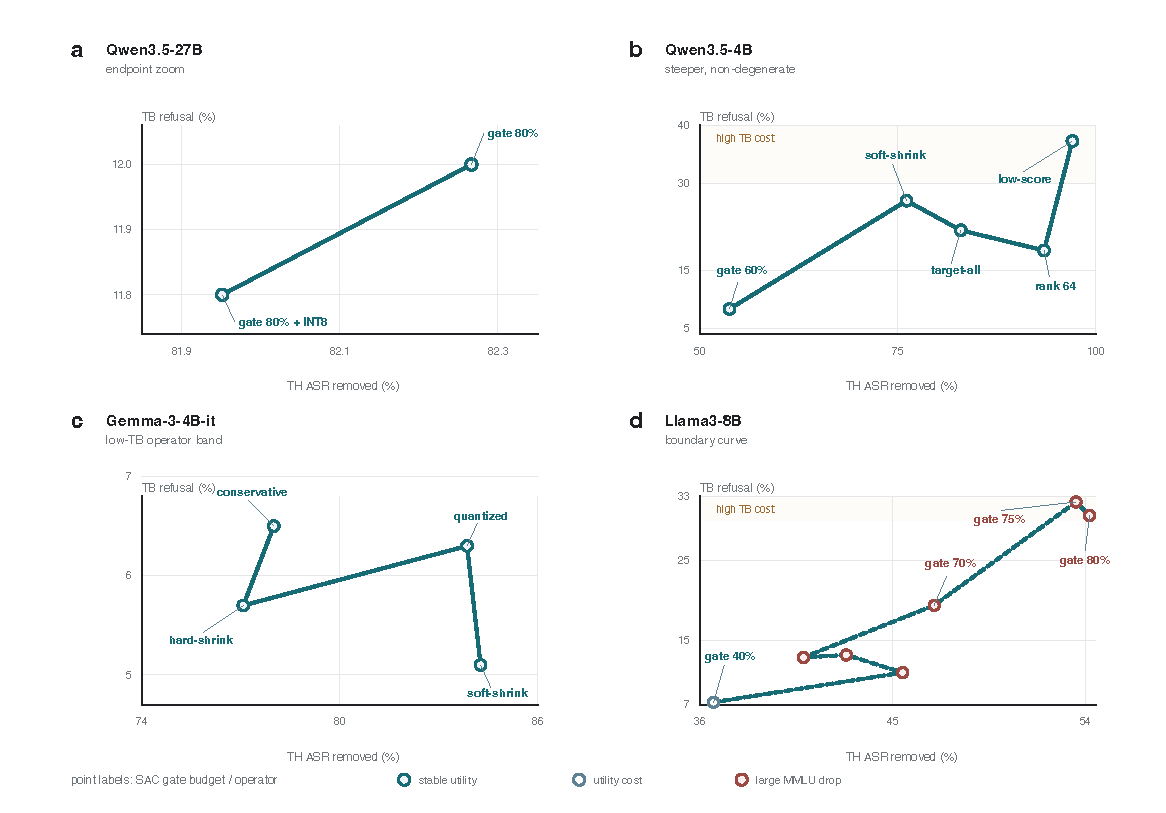
\includegraphics[width=0.98\textwidth]{figures/fig6_cross_model_frontiers.pdf}
\caption{Cross-model \sac{} frontier geometry. Each panel reports the same quantities but uses a panel-specific zoom so local structure is visible: x reports TH ASR removed relative to the backdoored adapter, and y reports triggered-benign refusal; both axes are shown as percentages, while the tables report the same rates on a 0--1 scale. Point labels identify either the SAC gate budget, materialization operator, or additional configuration. (a) Qwen27B zooms into the selected endpoint to separate the gate-only and gate-plus-INT8 variants. (b) Qwen4B shows a steeper but non-degenerate small-model frontier, including rank-64 and target-all-linear points. (c) Gemma forms a low-TB operator band. (d) Llama shows a higher-cost curve where stronger safety movement coincides with utility cost, indicated by marker fill.}
\label{fig:cross_model_frontiers}
\end{figure*}

\subsection{Qwen27B Provides the Cleanest Frontier Shift}

Qwen27B is the most favorable setting because \sac{} reduces triggered harmful attack success without relying on broad benign refusal.
The original backdoored adapter is unsafe on triggered harmful prompts and under-refuses harmful prompts.
\sac{} moves both quantities in the desired direction: TH decreases substantially and H refusal increases.
At the same time, TB and B refusal remain low and MMLU remains high under the 1,000-example protocol.
This is the target behavior for a post-hoc adapter defense: the model becomes substantially safer without collapsing into universal refusal.

The ablations support the selection mechanism.
Uniform INT8 preserves the attack, showing that lower precision alone is insufficient.
Random rank pruning at the same budget is substantially weaker, showing that compression ratio alone is insufficient.
Low-singular-value and magnitude-energy pruning also leave the attack active.
Adapter-state controls preserve the same pattern after loading or merging the adapter, so the effect is not an artifact of adapter loading state.
Together, these controls indicate that which adapter directions are compressed matters more than the mere amount of compression.
Figure~\ref{fig:mechanism} adds a more direct view of the selected gate.
The top of the \sac{} ranking is structured by layer and projection, the safety movement grows as more of this ranking is removed, and probe-refit gates overlap the selected gate more than random gates do.
This suggests that \sac{} is not merely pruning more; it repeatedly identifies a stable, localized subset of adapter directions whose removal tracks TH suppression.
The same selected direction set also reappears under an independently instantiated probe split: the reproduced 80\% gate drops the same 461 of 576 adapter directions as the main \method{SAC-alpha-80} gate (Jaccard 1.000), and its held-out evaluation remains close to the main 1,000-example row (Appendix Table~\ref{tab:supp_gate_repro}).
In panel (b), the teal curve is a single \sac{} alpha-budget sweep rather than separate methods at each point; the labeled 80\% endpoint corresponds to the selected \method{SAC-alpha-80} route used in the main tables, and the red point is the matched random-pruning control at the same budget.

\begin{figure*}[t]
\centering
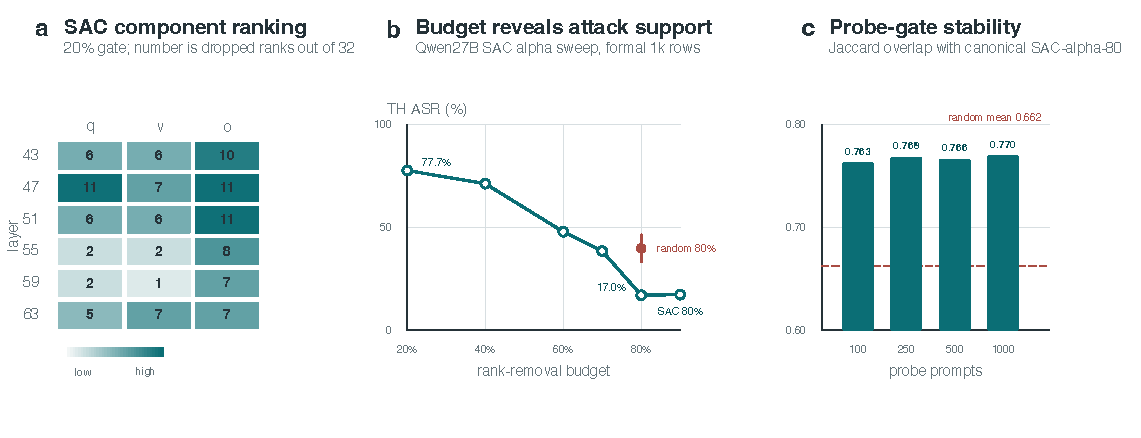
\includegraphics[width=0.98\textwidth]{figures/fig7_mechanism.pdf}
\caption{Qwen27B mechanism evidence from gate analysis. (a) The top 20\% of the \sac{} alpha ranking is concentrated across specific layer/projection cells; each number is the count of dropped ranks out of 32. (b) The teal curve is the \sac{} alpha-budget sweep along one ranking, with TH ASR shown as a percentage; the figure label ``SAC 80\%'' denotes the selected \method{SAC-alpha-80} endpoint, while the red point is ten-seed random pruning at the same 80\% budget. (c) Probe-size gates remain close to the selected \method{SAC-alpha-80} gate; the dashed line marks the mean overlap with random 80\% gates, and Jaccard overlap remains on a 0--1 scale. Taken together, the panels indicate a stable, localized subset of adapter directions whose removal tracks TH suppression.}
\label{fig:mechanism}
\end{figure*}

\subsection{Qwen4B Has a Steeper but Non-Degenerate Frontier}

Qwen4B shows the same intervention family in a smaller model.
The lowest-ASR row reaches TH 0.010, and several routes maintain MMLU near the original adapter.
The most aggressive rows induce high TB refusal, indicating that the trigger can become associated with refusal even for benign prompts.
The alpha sweep and additional rows show a structured frontier with non-degenerate operating points.
\method{SAC-alpha-60} has a normal-refusal profile (TB/B 0.083/0.081, close to the backdoor reference at 0.048/0.083) but only partial mitigation (TH 0.453).
Same-gate soft shrink and \method{SAC-alpha-70} move further along the frontier, lowering TH to 0.234/0.171 while raising TB to 0.270/0.304.
A clean-calibrated score-drop route reaches TH 0.029 with TB 0.373, after which the more aggressive layer routes move upward in TB refusal.
Uniform LoRA INT8 leaves TH at 0.974.
Additional Qwen4B rows further soften the over-refusal interpretation: a rank-64 setting reaches TH 0.064 with TB/B 0.184/0.114, and a target-all-linear setting reaches TH 0.167 with TB/B 0.219/0.062.
Moreover, Qwen4B clean-base and clean-adapter controls already show nontrivial triggered-benign refusal; in particular, clean-base TB is 0.480, indicating that the trigger string itself can induce refusal bias in this smaller model.
Thus, Qwen4B TB increases reflect small-model trigger sensitivity as well as the choice of \sac{} operating point.

This regime is qualitatively different from Qwen27B.
The lower-TH points substantially suppress the backdoor, and the additional rank-64 and target-all-linear points show that Qwen4B can avoid collapsing into universal refusal.
From a deployment perspective, the frontier is still less flat than Qwen27B: some aggressive points acquire a trigger-conditioned refusal artifact, so a user who can induce or accidentally include the trigger may cause benign requests to be refused.
Qwen4B therefore requires a more explicit operating-point choice than Qwen27B: lower TH is available, but the TB cost rises more quickly.

\subsection{Gemma Shows a Cross-Family Improvement}

Gemma-3-4B-it tests whether the same selection idea extends beyond Qwen.
The highlighted Gemma routes reduce TH from 0.973 to 0.157--0.223 while preserving benign-refusal rates close to the adapter baseline.
The reduction is smaller than Qwen27B because H refusal remains moderate and the utility baseline is lower.
Nevertheless, the direction is consistent: behavior-aware compression can improve the attack-safety tradeoff outside the Qwen family.

\subsection{Llama Reveals a High-Cost Regime}

Llama3-8B is the clearest high-cost setting in this study.
The \method{SAC-alpha-80} route reduces TH relative to the backdoored adapter while utility and benign refusal move along a higher-cost curve.
In the corresponding MMLU run, the alpha-budget sweep gives MMLU values 0.499/0.466/0.462/0.456/0.453/0.464/0.409 for 40/55/60/65/70/75/80\% alpha-rank budgets, so the lowest-TH alpha point is also the weakest utility point in that sweep.
Layer-adaptive variants move behavior within the same high-cost region.
Taken together, the cross-model results show that security-aware selection can produce substantial adapter-level mitigation and that the attainable frontier is model-dependent.
The present data make Llama the most direct stress test for the mechanism.
The observed pattern is consistent with two mechanism-level explanations: utility-bearing and trigger-bearing directions may be more entangled in the Llama adapter, and the component score distribution may be less concentrated, making the selected gate remove useful directions along with unsafe ones.
We treat this as evidence for heterogeneity in adapter geometry rather than as a complete causal account of the Llama pattern.

\subsection{Compression as Part of the Safety Surface}

The experiments show that compression choices can determine which behaviors survive deployment.
Two adapters with similar parameter budgets can have substantially different security profiles.
Uniform INT8 can preserve a backdoor, random pruning can partially reduce it, and behavior-aware selection can suppress it substantially.
Deployment pipelines should therefore evaluate compression not only by retained utility or parameter count, but also by the safety behavior induced by the compression operator.
